% ═══════════════════════════════════════════════════════════════════════
\section{La courbe de von Koch}
% ═══════════════════════════════════════════════════════════════════════

\begin{frame}{Figure 3.2 --- La construction}
  \small Étape $K_0$ : un segment de longueur $1$. On le partage en trois,
  on remplace le tiers central par les deux autres côtés d'un triangle
  équilatéral : $K_1$, quatre segments de longueur $\tfrac13$. On
  recommence sur chaque segment, et ainsi de suite.
  \FigBox[0.5\textheight]{%
    \begin{tikzpicture}[scale=5.5, courbe/.style={sectioncolor, line join=round, thick}]
      \foreach \n/\x/\y in {0/0/0, 1/0/-0.42, 2/0/-0.84, 3/1.25/0, 4/1.25/-0.42}{
        \begin{scope}[shift={(\x,\y)}]
          \input{figures/fractales/koch-\n.tikz}
          \node[etiq, left, sectioncolor] at (-0.02,0.04) {$K_{\n}$};
        \end{scope}}
      \begin{scope}[shift={(1.25,-0.84)}, courbe/.style={sectioncolor, line join=round, thin}]
        % Courbe de von Koch, étape 5
% Fichier généré par generer.py : ne pas modifier à la main.
\draw[courbe]
  (0,0) -- (0.0041,0) -- (0.0062,0.0036) -- (0.0082,0) -- (0.0123,0) -- (0.0144,0.0036) --
  (0.0123,0.0071) -- (0.0165,0.0071) -- (0.0185,0.0107) -- (0.0206,0.0071) -- (0.0247,0.0071) -- (0.0226,0.0036) --
  (0.0247,0) -- (0.0288,0) -- (0.0309,0.0036) -- (0.0329,0) -- (0.037,0) -- (0.0391,0.0036) --
  (0.037,0.0071) -- (0.0412,0.0071) -- (0.0432,0.0107) -- (0.0412,0.0143) -- (0.037,0.0143) -- (0.0391,0.0178) --
  (0.037,0.0214) -- (0.0412,0.0214) -- (0.0432,0.0249) -- (0.0453,0.0214) -- (0.0494,0.0214) -- (0.0514,0.0249) --
  (0.0494,0.0285) -- (0.0535,0.0285) -- (0.0556,0.0321) -- (0.0576,0.0285) -- (0.0617,0.0285) -- (0.0597,0.0249) --
  (0.0617,0.0214) -- (0.0658,0.0214) -- (0.0679,0.0249) -- (0.07,0.0214) -- (0.0741,0.0214) -- (0.072,0.0178) --
  (0.0741,0.0143) -- (0.07,0.0143) -- (0.0679,0.0107) -- (0.07,0.0071) -- (0.0741,0.0071) -- (0.072,0.0036) --
  (0.0741,0) -- (0.0782,0) -- (0.0802,0.0036) -- (0.0823,0) -- (0.0864,0) -- (0.0885,0.0036) --
  (0.0864,0.0071) -- (0.0905,0.0071) -- (0.0926,0.0107) -- (0.0947,0.0071) -- (0.0988,0.0071) -- (0.0967,0.0036) --
  (0.0988,0) -- (0.1029,0) -- (0.1049,0.0036) -- (0.107,0) -- (0.1111,0) -- (0.1132,0.0036) --
  (0.1111,0.0071) -- (0.1152,0.0071) -- (0.1173,0.0107) -- (0.1152,0.0143) -- (0.1111,0.0143) -- (0.1132,0.0178) --
  (0.1111,0.0214) -- (0.1152,0.0214) -- (0.1173,0.0249) -- (0.1193,0.0214) -- (0.1235,0.0214) -- (0.1255,0.0249) --
  (0.1235,0.0285) -- (0.1276,0.0285) -- (0.1296,0.0321) -- (0.1276,0.0356) -- (0.1235,0.0356) -- (0.1255,0.0392) --
  (0.1235,0.0428) -- (0.1193,0.0428) -- (0.1173,0.0392) -- (0.1152,0.0428) -- (0.1111,0.0428) -- (0.1132,0.0463) --
  (0.1111,0.0499) -- (0.1152,0.0499) -- (0.1173,0.0535) -- (0.1152,0.057) -- (0.1111,0.057) -- (0.1132,0.0606) --
  (0.1111,0.0642) -- (0.1152,0.0642) -- (0.1173,0.0677) -- (0.1193,0.0642) -- (0.1235,0.0642) -- (0.1255,0.0677) --
  (0.1235,0.0713) -- (0.1276,0.0713) -- (0.1296,0.0748) -- (0.1317,0.0713) -- (0.1358,0.0713) -- (0.1337,0.0677) --
  (0.1358,0.0642) -- (0.1399,0.0642) -- (0.142,0.0677) -- (0.144,0.0642) -- (0.1481,0.0642) -- (0.1502,0.0677) --
  (0.1481,0.0713) -- (0.1523,0.0713) -- (0.1543,0.0748) -- (0.1523,0.0784) -- (0.1481,0.0784) -- (0.1502,0.082) --
  (0.1481,0.0855) -- (0.1523,0.0855) -- (0.1543,0.0891) -- (0.1564,0.0855) -- (0.1605,0.0855) -- (0.1626,0.0891) --
  (0.1605,0.0927) -- (0.1646,0.0927) -- (0.1667,0.0962) -- (0.1687,0.0927) -- (0.1728,0.0927) -- (0.1708,0.0891) --
  (0.1728,0.0855) -- (0.177,0.0855) -- (0.179,0.0891) -- (0.1811,0.0855) -- (0.1852,0.0855) -- (0.1831,0.082) --
  (0.1852,0.0784) -- (0.1811,0.0784) -- (0.179,0.0748) -- (0.1811,0.0713) -- (0.1852,0.0713) -- (0.1831,0.0677) --
  (0.1852,0.0642) -- (0.1893,0.0642) -- (0.1914,0.0677) -- (0.1934,0.0642) -- (0.1975,0.0642) -- (0.1996,0.0677) --
  (0.1975,0.0713) -- (0.2016,0.0713) -- (0.2037,0.0748) -- (0.2058,0.0713) -- (0.2099,0.0713) -- (0.2078,0.0677) --
  (0.2099,0.0642) -- (0.214,0.0642) -- (0.216,0.0677) -- (0.2181,0.0642) -- (0.2222,0.0642) -- (0.2202,0.0606) --
  (0.2222,0.057) -- (0.2181,0.057) -- (0.216,0.0535) -- (0.2181,0.0499) -- (0.2222,0.0499) -- (0.2202,0.0463) --
  (0.2222,0.0428) -- (0.2181,0.0428) -- (0.216,0.0392) -- (0.214,0.0428) -- (0.2099,0.0428) -- (0.2078,0.0392) --
  (0.2099,0.0356) -- (0.2058,0.0356) -- (0.2037,0.0321) -- (0.2058,0.0285) -- (0.2099,0.0285) -- (0.2078,0.0249) --
  (0.2099,0.0214) -- (0.214,0.0214) -- (0.216,0.0249) -- (0.2181,0.0214) -- (0.2222,0.0214) -- (0.2202,0.0178) --
  (0.2222,0.0143) -- (0.2181,0.0143) -- (0.216,0.0107) -- (0.2181,0.0071) -- (0.2222,0.0071) -- (0.2202,0.0036) --
  (0.2222,0) -- (0.2263,0) -- (0.2284,0.0036) -- (0.2305,0) -- (0.2346,0) -- (0.2366,0.0036) --
  (0.2346,0.0071) -- (0.2387,0.0071) -- (0.2407,0.0107) -- (0.2428,0.0071) -- (0.2469,0.0071) -- (0.2449,0.0036) --
  (0.2469,0) -- (0.251,0) -- (0.2531,0.0036) -- (0.2551,0) -- (0.2593,0) -- (0.2613,0.0036) --
  (0.2593,0.0071) -- (0.2634,0.0071) -- (0.2654,0.0107) -- (0.2634,0.0143) -- (0.2593,0.0143) -- (0.2613,0.0178) --
  (0.2593,0.0214) -- (0.2634,0.0214) -- (0.2654,0.0249) -- (0.2675,0.0214) -- (0.2716,0.0214) -- (0.2737,0.0249) --
  (0.2716,0.0285) -- (0.2757,0.0285) -- (0.2778,0.0321) -- (0.2798,0.0285) -- (0.284,0.0285) -- (0.2819,0.0249) --
  (0.284,0.0214) -- (0.2881,0.0214) -- (0.2901,0.0249) -- (0.2922,0.0214) -- (0.2963,0.0214) -- (0.2942,0.0178) --
  (0.2963,0.0143) -- (0.2922,0.0143) -- (0.2901,0.0107) -- (0.2922,0.0071) -- (0.2963,0.0071) -- (0.2942,0.0036) --
  (0.2963,0) -- (0.3004,0) -- (0.3025,0.0036) -- (0.3045,0) -- (0.3086,0) -- (0.3107,0.0036) --
  (0.3086,0.0071) -- (0.3128,0.0071) -- (0.3148,0.0107) -- (0.3169,0.0071) -- (0.321,0.0071) -- (0.3189,0.0036) --
  (0.321,0) -- (0.3251,0) -- (0.3272,0.0036) -- (0.3292,0) -- (0.3333,0) -- (0.3354,0.0036) --
  (0.3333,0.0071) -- (0.3374,0.0071) -- (0.3395,0.0107) -- (0.3374,0.0143) -- (0.3333,0.0143) -- (0.3354,0.0178) --
  (0.3333,0.0214) -- (0.3374,0.0214) -- (0.3395,0.0249) -- (0.3416,0.0214) -- (0.3457,0.0214) -- (0.3477,0.0249) --
  (0.3457,0.0285) -- (0.3498,0.0285) -- (0.3519,0.0321) -- (0.3498,0.0356) -- (0.3457,0.0356) -- (0.3477,0.0392) --
  (0.3457,0.0428) -- (0.3416,0.0428) -- (0.3395,0.0392) -- (0.3374,0.0428) -- (0.3333,0.0428) -- (0.3354,0.0463) --
  (0.3333,0.0499) -- (0.3374,0.0499) -- (0.3395,0.0535) -- (0.3374,0.057) -- (0.3333,0.057) -- (0.3354,0.0606) --
  (0.3333,0.0642) -- (0.3374,0.0642) -- (0.3395,0.0677) -- (0.3416,0.0642) -- (0.3457,0.0642) -- (0.3477,0.0677) --
  (0.3457,0.0713) -- (0.3498,0.0713) -- (0.3519,0.0748) -- (0.3539,0.0713) -- (0.358,0.0713) -- (0.356,0.0677) --
  (0.358,0.0642) -- (0.3621,0.0642) -- (0.3642,0.0677) -- (0.3663,0.0642) -- (0.3704,0.0642) -- (0.3724,0.0677) --
  (0.3704,0.0713) -- (0.3745,0.0713) -- (0.3765,0.0748) -- (0.3745,0.0784) -- (0.3704,0.0784) -- (0.3724,0.082) --
  (0.3704,0.0855) -- (0.3745,0.0855) -- (0.3765,0.0891) -- (0.3786,0.0855) -- (0.3827,0.0855) -- (0.3848,0.0891) --
  (0.3827,0.0927) -- (0.3868,0.0927) -- (0.3889,0.0962) -- (0.3868,0.0998) -- (0.3827,0.0998) -- (0.3848,0.1034) --
  (0.3827,0.1069) -- (0.3786,0.1069) -- (0.3765,0.1034) -- (0.3745,0.1069) -- (0.3704,0.1069) -- (0.3724,0.1105) --
  (0.3704,0.114) -- (0.3745,0.114) -- (0.3765,0.1176) -- (0.3745,0.1212) -- (0.3704,0.1212) -- (0.3724,0.1247) --
  (0.3704,0.1283) -- (0.3663,0.1283) -- (0.3642,0.1247) -- (0.3621,0.1283) -- (0.358,0.1283) -- (0.356,0.1247) --
  (0.358,0.1212) -- (0.3539,0.1212) -- (0.3519,0.1176) -- (0.3498,0.1212) -- (0.3457,0.1212) -- (0.3477,0.1247) --
  (0.3457,0.1283) -- (0.3416,0.1283) -- (0.3395,0.1247) -- (0.3374,0.1283) -- (0.3333,0.1283) -- (0.3354,0.1319) --
  (0.3333,0.1354) -- (0.3374,0.1354) -- (0.3395,0.139) -- (0.3374,0.1426) -- (0.3333,0.1426) -- (0.3354,0.1461) --
  (0.3333,0.1497) -- (0.3374,0.1497) -- (0.3395,0.1532) -- (0.3416,0.1497) -- (0.3457,0.1497) -- (0.3477,0.1532) --
  (0.3457,0.1568) -- (0.3498,0.1568) -- (0.3519,0.1604) -- (0.3498,0.1639) -- (0.3457,0.1639) -- (0.3477,0.1675) --
  (0.3457,0.1711) -- (0.3416,0.1711) -- (0.3395,0.1675) -- (0.3374,0.1711) -- (0.3333,0.1711) -- (0.3354,0.1746) --
  (0.3333,0.1782) -- (0.3374,0.1782) -- (0.3395,0.1818) -- (0.3374,0.1853) -- (0.3333,0.1853) -- (0.3354,0.1889) --
  (0.3333,0.1925) -- (0.3374,0.1925) -- (0.3395,0.196) -- (0.3416,0.1925) -- (0.3457,0.1925) -- (0.3477,0.196) --
  (0.3457,0.1996) -- (0.3498,0.1996) -- (0.3519,0.2031) -- (0.3539,0.1996) -- (0.358,0.1996) -- (0.356,0.196) --
  (0.358,0.1925) -- (0.3621,0.1925) -- (0.3642,0.196) -- (0.3663,0.1925) -- (0.3704,0.1925) -- (0.3724,0.196) --
  (0.3704,0.1996) -- (0.3745,0.1996) -- (0.3765,0.2031) -- (0.3745,0.2067) -- (0.3704,0.2067) -- (0.3724,0.2103) --
  (0.3704,0.2138) -- (0.3745,0.2138) -- (0.3765,0.2174) -- (0.3786,0.2138) -- (0.3827,0.2138) -- (0.3848,0.2174) --
  (0.3827,0.221) -- (0.3868,0.221) -- (0.3889,0.2245) -- (0.3909,0.221) -- (0.3951,0.221) -- (0.393,0.2174) --
  (0.3951,0.2138) -- (0.3992,0.2138) -- (0.4012,0.2174) -- (0.4033,0.2138) -- (0.4074,0.2138) -- (0.4053,0.2103) --
  (0.4074,0.2067) -- (0.4033,0.2067) -- (0.4012,0.2031) -- (0.4033,0.1996) -- (0.4074,0.1996) -- (0.4053,0.196) --
  (0.4074,0.1925) -- (0.4115,0.1925) -- (0.4136,0.196) -- (0.4156,0.1925) -- (0.4198,0.1925) -- (0.4218,0.196) --
  (0.4198,0.1996) -- (0.4239,0.1996) -- (0.4259,0.2031) -- (0.428,0.1996) -- (0.4321,0.1996) -- (0.43,0.196) --
  (0.4321,0.1925) -- (0.4362,0.1925) -- (0.4383,0.196) -- (0.4403,0.1925) -- (0.4444,0.1925) -- (0.4465,0.196) --
  (0.4444,0.1996) -- (0.4486,0.1996) -- (0.4506,0.2031) -- (0.4486,0.2067) -- (0.4444,0.2067) -- (0.4465,0.2103) --
  (0.4444,0.2138) -- (0.4486,0.2138) -- (0.4506,0.2174) -- (0.4527,0.2138) -- (0.4568,0.2138) -- (0.4588,0.2174) --
  (0.4568,0.221) -- (0.4609,0.221) -- (0.463,0.2245) -- (0.4609,0.2281) -- (0.4568,0.2281) -- (0.4588,0.2317) --
  (0.4568,0.2352) -- (0.4527,0.2352) -- (0.4506,0.2317) -- (0.4486,0.2352) -- (0.4444,0.2352) -- (0.4465,0.2388) --
  (0.4444,0.2423) -- (0.4486,0.2423) -- (0.4506,0.2459) -- (0.4486,0.2495) -- (0.4444,0.2495) -- (0.4465,0.253) --
  (0.4444,0.2566) -- (0.4486,0.2566) -- (0.4506,0.2602) -- (0.4527,0.2566) -- (0.4568,0.2566) -- (0.4588,0.2602) --
  (0.4568,0.2637) -- (0.4609,0.2637) -- (0.463,0.2673) -- (0.465,0.2637) -- (0.4691,0.2637) -- (0.4671,0.2602) --
  (0.4691,0.2566) -- (0.4733,0.2566) -- (0.4753,0.2602) -- (0.4774,0.2566) -- (0.4815,0.2566) -- (0.4835,0.2602) --
  (0.4815,0.2637) -- (0.4856,0.2637) -- (0.4877,0.2673) -- (0.4856,0.2709) -- (0.4815,0.2709) -- (0.4835,0.2744) --
  (0.4815,0.278) -- (0.4856,0.278) -- (0.4877,0.2815) -- (0.4897,0.278) -- (0.4938,0.278) -- (0.4959,0.2815) --
  (0.4938,0.2851) -- (0.4979,0.2851) -- (0.5,0.2887) -- (0.5021,0.2851) -- (0.5062,0.2851) -- (0.5041,0.2815) --
  (0.5062,0.278) -- (0.5103,0.278) -- (0.5123,0.2815) -- (0.5144,0.278) -- (0.5185,0.278) -- (0.5165,0.2744) --
  (0.5185,0.2709) -- (0.5144,0.2709) -- (0.5123,0.2673) -- (0.5144,0.2637) -- (0.5185,0.2637) -- (0.5165,0.2602) --
  (0.5185,0.2566) -- (0.5226,0.2566) -- (0.5247,0.2602) -- (0.5267,0.2566) -- (0.5309,0.2566) -- (0.5329,0.2602) --
  (0.5309,0.2637) -- (0.535,0.2637) -- (0.537,0.2673) -- (0.5391,0.2637) -- (0.5432,0.2637) -- (0.5412,0.2602) --
  (0.5432,0.2566) -- (0.5473,0.2566) -- (0.5494,0.2602) -- (0.5514,0.2566) -- (0.5556,0.2566) -- (0.5535,0.253) --
  (0.5556,0.2495) -- (0.5514,0.2495) -- (0.5494,0.2459) -- (0.5514,0.2423) -- (0.5556,0.2423) -- (0.5535,0.2388) --
  (0.5556,0.2352) -- (0.5514,0.2352) -- (0.5494,0.2317) -- (0.5473,0.2352) -- (0.5432,0.2352) -- (0.5412,0.2317) --
  (0.5432,0.2281) -- (0.5391,0.2281) -- (0.537,0.2245) -- (0.5391,0.221) -- (0.5432,0.221) -- (0.5412,0.2174) --
  (0.5432,0.2138) -- (0.5473,0.2138) -- (0.5494,0.2174) -- (0.5514,0.2138) -- (0.5556,0.2138) -- (0.5535,0.2103) --
  (0.5556,0.2067) -- (0.5514,0.2067) -- (0.5494,0.2031) -- (0.5514,0.1996) -- (0.5556,0.1996) -- (0.5535,0.196) --
  (0.5556,0.1925) -- (0.5597,0.1925) -- (0.5617,0.196) -- (0.5638,0.1925) -- (0.5679,0.1925) -- (0.57,0.196) --
  (0.5679,0.1996) -- (0.572,0.1996) -- (0.5741,0.2031) -- (0.5761,0.1996) -- (0.5802,0.1996) -- (0.5782,0.196) --
  (0.5802,0.1925) -- (0.5844,0.1925) -- (0.5864,0.196) -- (0.5885,0.1925) -- (0.5926,0.1925) -- (0.5947,0.196) --
  (0.5926,0.1996) -- (0.5967,0.1996) -- (0.5988,0.2031) -- (0.5967,0.2067) -- (0.5926,0.2067) -- (0.5947,0.2103) --
  (0.5926,0.2138) -- (0.5967,0.2138) -- (0.5988,0.2174) -- (0.6008,0.2138) -- (0.6049,0.2138) -- (0.607,0.2174) --
  (0.6049,0.221) -- (0.6091,0.221) -- (0.6111,0.2245) -- (0.6132,0.221) -- (0.6173,0.221) -- (0.6152,0.2174) --
  (0.6173,0.2138) -- (0.6214,0.2138) -- (0.6235,0.2174) -- (0.6255,0.2138) -- (0.6296,0.2138) -- (0.6276,0.2103) --
  (0.6296,0.2067) -- (0.6255,0.2067) -- (0.6235,0.2031) -- (0.6255,0.1996) -- (0.6296,0.1996) -- (0.6276,0.196) --
  (0.6296,0.1925) -- (0.6337,0.1925) -- (0.6358,0.196) -- (0.6379,0.1925) -- (0.642,0.1925) -- (0.644,0.196) --
  (0.642,0.1996) -- (0.6461,0.1996) -- (0.6481,0.2031) -- (0.6502,0.1996) -- (0.6543,0.1996) -- (0.6523,0.196) --
  (0.6543,0.1925) -- (0.6584,0.1925) -- (0.6605,0.196) -- (0.6626,0.1925) -- (0.6667,0.1925) -- (0.6646,0.1889) --
  (0.6667,0.1853) -- (0.6626,0.1853) -- (0.6605,0.1818) -- (0.6626,0.1782) -- (0.6667,0.1782) -- (0.6646,0.1746) --
  (0.6667,0.1711) -- (0.6626,0.1711) -- (0.6605,0.1675) -- (0.6584,0.1711) -- (0.6543,0.1711) -- (0.6523,0.1675) --
  (0.6543,0.1639) -- (0.6502,0.1639) -- (0.6481,0.1604) -- (0.6502,0.1568) -- (0.6543,0.1568) -- (0.6523,0.1532) --
  (0.6543,0.1497) -- (0.6584,0.1497) -- (0.6605,0.1532) -- (0.6626,0.1497) -- (0.6667,0.1497) -- (0.6646,0.1461) --
  (0.6667,0.1426) -- (0.6626,0.1426) -- (0.6605,0.139) -- (0.6626,0.1354) -- (0.6667,0.1354) -- (0.6646,0.1319) --
  (0.6667,0.1283) -- (0.6626,0.1283) -- (0.6605,0.1247) -- (0.6584,0.1283) -- (0.6543,0.1283) -- (0.6523,0.1247) --
  (0.6543,0.1212) -- (0.6502,0.1212) -- (0.6481,0.1176) -- (0.6461,0.1212) -- (0.642,0.1212) -- (0.644,0.1247) --
  (0.642,0.1283) -- (0.6379,0.1283) -- (0.6358,0.1247) -- (0.6337,0.1283) -- (0.6296,0.1283) -- (0.6276,0.1247) --
  (0.6296,0.1212) -- (0.6255,0.1212) -- (0.6235,0.1176) -- (0.6255,0.114) -- (0.6296,0.114) -- (0.6276,0.1105) --
  (0.6296,0.1069) -- (0.6255,0.1069) -- (0.6235,0.1034) -- (0.6214,0.1069) -- (0.6173,0.1069) -- (0.6152,0.1034) --
  (0.6173,0.0998) -- (0.6132,0.0998) -- (0.6111,0.0962) -- (0.6132,0.0927) -- (0.6173,0.0927) -- (0.6152,0.0891) --
  (0.6173,0.0855) -- (0.6214,0.0855) -- (0.6235,0.0891) -- (0.6255,0.0855) -- (0.6296,0.0855) -- (0.6276,0.082) --
  (0.6296,0.0784) -- (0.6255,0.0784) -- (0.6235,0.0748) -- (0.6255,0.0713) -- (0.6296,0.0713) -- (0.6276,0.0677) --
  (0.6296,0.0642) -- (0.6337,0.0642) -- (0.6358,0.0677) -- (0.6379,0.0642) -- (0.642,0.0642) -- (0.644,0.0677) --
  (0.642,0.0713) -- (0.6461,0.0713) -- (0.6481,0.0748) -- (0.6502,0.0713) -- (0.6543,0.0713) -- (0.6523,0.0677) --
  (0.6543,0.0642) -- (0.6584,0.0642) -- (0.6605,0.0677) -- (0.6626,0.0642) -- (0.6667,0.0642) -- (0.6646,0.0606) --
  (0.6667,0.057) -- (0.6626,0.057) -- (0.6605,0.0535) -- (0.6626,0.0499) -- (0.6667,0.0499) -- (0.6646,0.0463) --
  (0.6667,0.0428) -- (0.6626,0.0428) -- (0.6605,0.0392) -- (0.6584,0.0428) -- (0.6543,0.0428) -- (0.6523,0.0392) --
  (0.6543,0.0356) -- (0.6502,0.0356) -- (0.6481,0.0321) -- (0.6502,0.0285) -- (0.6543,0.0285) -- (0.6523,0.0249) --
  (0.6543,0.0214) -- (0.6584,0.0214) -- (0.6605,0.0249) -- (0.6626,0.0214) -- (0.6667,0.0214) -- (0.6646,0.0178) --
  (0.6667,0.0143) -- (0.6626,0.0143) -- (0.6605,0.0107) -- (0.6626,0.0071) -- (0.6667,0.0071) -- (0.6646,0.0036) --
  (0.6667,0) -- (0.6708,0) -- (0.6728,0.0036) -- (0.6749,0) -- (0.679,0) -- (0.6811,0.0036) --
  (0.679,0.0071) -- (0.6831,0.0071) -- (0.6852,0.0107) -- (0.6872,0.0071) -- (0.6914,0.0071) -- (0.6893,0.0036) --
  (0.6914,0) -- (0.6955,0) -- (0.6975,0.0036) -- (0.6996,0) -- (0.7037,0) -- (0.7058,0.0036) --
  (0.7037,0.0071) -- (0.7078,0.0071) -- (0.7099,0.0107) -- (0.7078,0.0143) -- (0.7037,0.0143) -- (0.7058,0.0178) --
  (0.7037,0.0214) -- (0.7078,0.0214) -- (0.7099,0.0249) -- (0.7119,0.0214) -- (0.716,0.0214) -- (0.7181,0.0249) --
  (0.716,0.0285) -- (0.7202,0.0285) -- (0.7222,0.0321) -- (0.7243,0.0285) -- (0.7284,0.0285) -- (0.7263,0.0249) --
  (0.7284,0.0214) -- (0.7325,0.0214) -- (0.7346,0.0249) -- (0.7366,0.0214) -- (0.7407,0.0214) -- (0.7387,0.0178) --
  (0.7407,0.0143) -- (0.7366,0.0143) -- (0.7346,0.0107) -- (0.7366,0.0071) -- (0.7407,0.0071) -- (0.7387,0.0036) --
  (0.7407,0) -- (0.7449,0) -- (0.7469,0.0036) -- (0.749,0) -- (0.7531,0) -- (0.7551,0.0036) --
  (0.7531,0.0071) -- (0.7572,0.0071) -- (0.7593,0.0107) -- (0.7613,0.0071) -- (0.7654,0.0071) -- (0.7634,0.0036) --
  (0.7654,0) -- (0.7695,0) -- (0.7716,0.0036) -- (0.7737,0) -- (0.7778,0) -- (0.7798,0.0036) --
  (0.7778,0.0071) -- (0.7819,0.0071) -- (0.784,0.0107) -- (0.7819,0.0143) -- (0.7778,0.0143) -- (0.7798,0.0178) --
  (0.7778,0.0214) -- (0.7819,0.0214) -- (0.784,0.0249) -- (0.786,0.0214) -- (0.7901,0.0214) -- (0.7922,0.0249) --
  (0.7901,0.0285) -- (0.7942,0.0285) -- (0.7963,0.0321) -- (0.7942,0.0356) -- (0.7901,0.0356) -- (0.7922,0.0392) --
  (0.7901,0.0428) -- (0.786,0.0428) -- (0.784,0.0392) -- (0.7819,0.0428) -- (0.7778,0.0428) -- (0.7798,0.0463) --
  (0.7778,0.0499) -- (0.7819,0.0499) -- (0.784,0.0535) -- (0.7819,0.057) -- (0.7778,0.057) -- (0.7798,0.0606) --
  (0.7778,0.0642) -- (0.7819,0.0642) -- (0.784,0.0677) -- (0.786,0.0642) -- (0.7901,0.0642) -- (0.7922,0.0677) --
  (0.7901,0.0713) -- (0.7942,0.0713) -- (0.7963,0.0748) -- (0.7984,0.0713) -- (0.8025,0.0713) -- (0.8004,0.0677) --
  (0.8025,0.0642) -- (0.8066,0.0642) -- (0.8086,0.0677) -- (0.8107,0.0642) -- (0.8148,0.0642) -- (0.8169,0.0677) --
  (0.8148,0.0713) -- (0.8189,0.0713) -- (0.821,0.0748) -- (0.8189,0.0784) -- (0.8148,0.0784) -- (0.8169,0.082) --
  (0.8148,0.0855) -- (0.8189,0.0855) -- (0.821,0.0891) -- (0.823,0.0855) -- (0.8272,0.0855) -- (0.8292,0.0891) --
  (0.8272,0.0927) -- (0.8313,0.0927) -- (0.8333,0.0962) -- (0.8354,0.0927) -- (0.8395,0.0927) -- (0.8374,0.0891) --
  (0.8395,0.0855) -- (0.8436,0.0855) -- (0.8457,0.0891) -- (0.8477,0.0855) -- (0.8519,0.0855) -- (0.8498,0.082) --
  (0.8519,0.0784) -- (0.8477,0.0784) -- (0.8457,0.0748) -- (0.8477,0.0713) -- (0.8519,0.0713) -- (0.8498,0.0677) --
  (0.8519,0.0642) -- (0.856,0.0642) -- (0.858,0.0677) -- (0.8601,0.0642) -- (0.8642,0.0642) -- (0.8663,0.0677) --
  (0.8642,0.0713) -- (0.8683,0.0713) -- (0.8704,0.0748) -- (0.8724,0.0713) -- (0.8765,0.0713) -- (0.8745,0.0677) --
  (0.8765,0.0642) -- (0.8807,0.0642) -- (0.8827,0.0677) -- (0.8848,0.0642) -- (0.8889,0.0642) -- (0.8868,0.0606) --
  (0.8889,0.057) -- (0.8848,0.057) -- (0.8827,0.0535) -- (0.8848,0.0499) -- (0.8889,0.0499) -- (0.8868,0.0463) --
  (0.8889,0.0428) -- (0.8848,0.0428) -- (0.8827,0.0392) -- (0.8807,0.0428) -- (0.8765,0.0428) -- (0.8745,0.0392) --
  (0.8765,0.0356) -- (0.8724,0.0356) -- (0.8704,0.0321) -- (0.8724,0.0285) -- (0.8765,0.0285) -- (0.8745,0.0249) --
  (0.8765,0.0214) -- (0.8807,0.0214) -- (0.8827,0.0249) -- (0.8848,0.0214) -- (0.8889,0.0214) -- (0.8868,0.0178) --
  (0.8889,0.0143) -- (0.8848,0.0143) -- (0.8827,0.0107) -- (0.8848,0.0071) -- (0.8889,0.0071) -- (0.8868,0.0036) --
  (0.8889,0) -- (0.893,0) -- (0.8951,0.0036) -- (0.8971,0) -- (0.9012,0) -- (0.9033,0.0036) --
  (0.9012,0.0071) -- (0.9053,0.0071) -- (0.9074,0.0107) -- (0.9095,0.0071) -- (0.9136,0.0071) -- (0.9115,0.0036) --
  (0.9136,0) -- (0.9177,0) -- (0.9198,0.0036) -- (0.9218,0) -- (0.9259,0) -- (0.928,0.0036) --
  (0.9259,0.0071) -- (0.93,0.0071) -- (0.9321,0.0107) -- (0.93,0.0143) -- (0.9259,0.0143) -- (0.928,0.0178) --
  (0.9259,0.0214) -- (0.93,0.0214) -- (0.9321,0.0249) -- (0.9342,0.0214) -- (0.9383,0.0214) -- (0.9403,0.0249) --
  (0.9383,0.0285) -- (0.9424,0.0285) -- (0.9444,0.0321) -- (0.9465,0.0285) -- (0.9506,0.0285) -- (0.9486,0.0249) --
  (0.9506,0.0214) -- (0.9547,0.0214) -- (0.9568,0.0249) -- (0.9588,0.0214) -- (0.963,0.0214) -- (0.9609,0.0178) --
  (0.963,0.0143) -- (0.9588,0.0143) -- (0.9568,0.0107) -- (0.9588,0.0071) -- (0.963,0.0071) -- (0.9609,0.0036) --
  (0.963,0) -- (0.9671,0) -- (0.9691,0.0036) -- (0.9712,0) -- (0.9753,0) -- (0.9774,0.0036) --
  (0.9753,0.0071) -- (0.9794,0.0071) -- (0.9815,0.0107) -- (0.9835,0.0071) -- (0.9877,0.0071) -- (0.9856,0.0036) --
  (0.9877,0) -- (0.9918,0) -- (0.9938,0.0036) -- (0.9959,0) -- (1,0);

        \node[etiq, left, sectioncolor] at (-0.02,0.04) {$K_{5}$};
      \end{scope}
    \end{tikzpicture}}
  \small La courbe de von Koch $K$ est la figure limite. Le sens de cette
  limite, dans $\big(\Comp{\R^2},\dH\big)$, sera justifié en section 6.
\end{frame}

\begin{frame}{Première propriété : sa longueur est infinie}
  \small À chaque étape, chaque segment est remplacé par quatre segments
  trois fois plus courts : la longueur est multipliée par $\tfrac43$.
  \[
    L_n = \left(\frac43\right)^{\!n} \xrightarrow[n\to\infty]{} \infty .
  \]
  \begin{itemize}
    \item $L_{10}\approx\num{17.8}$ ; $L_{50}\approx\num{1.8e6}$.
    \item Si $K_0$ mesure un centimètre, $K_{50}$ est plus longue que la
      distance de Québec à Montréal --- et pourtant la figure tient sur
      un timbre-poste.
    \item Aucune longueur finie ne peut être attribuée à $K$.
  \end{itemize}
\end{frame}

\begin{frame}{Figure 3.3 --- Deuxième propriété : aucune tangente}
  \FigBox[0.5\textheight]{%
    \begin{tikzpicture}
      \begin{scope}[xscale=2.1, yscale=1.4]
        \draw[axe] (-0.1,0) -- (2.2,0);
        \draw[sectioncolor, thick, domain=0:2, samples=60, smooth]
          plot (\x, {1.2*sin(deg(\x*1.4))});
        \draw[firebrick3, thick] (0.5,0.79) rectangle (0.7,0.99);
        \node[etiq, sectioncolor] at (1.1,1.55) {une courbe lisse};
      \end{scope}
      \begin{scope}[shift={(5.6,0)}, xscale=2.1, yscale=1.4]
        \draw[firebrick3, thick] (0,0) rectangle (1.5,1.5);
        \clip (0,0) rectangle (1.5,1.5);
        \draw[sectioncolor, thick, domain=0.5:0.7, samples=40, smooth]
          plot ({(\x-0.5)/0.2*1.5}, {(1.2*sin(deg(1.4*\x))-0.79)/0.2*1.5});
      \end{scope}
      \node[etiq, sectioncolor] at (7.18,2.45) {agrandie : presque une droite};
      \draw[fleche, firebrick3!70] (1.5,1.4) to[bend left=15] (5.5,1.6);
      \begin{scope}[shift={(0,-3.4)}, scale=4.2, courbe/.style={sectioncolor, line join=round, thick}]
        % Courbe de von Koch, étape 5
% Fichier généré par generer.py : ne pas modifier à la main.
\draw[courbe]
  (0,0) -- (0.0041,0) -- (0.0062,0.0036) -- (0.0082,0) -- (0.0123,0) -- (0.0144,0.0036) --
  (0.0123,0.0071) -- (0.0165,0.0071) -- (0.0185,0.0107) -- (0.0206,0.0071) -- (0.0247,0.0071) -- (0.0226,0.0036) --
  (0.0247,0) -- (0.0288,0) -- (0.0309,0.0036) -- (0.0329,0) -- (0.037,0) -- (0.0391,0.0036) --
  (0.037,0.0071) -- (0.0412,0.0071) -- (0.0432,0.0107) -- (0.0412,0.0143) -- (0.037,0.0143) -- (0.0391,0.0178) --
  (0.037,0.0214) -- (0.0412,0.0214) -- (0.0432,0.0249) -- (0.0453,0.0214) -- (0.0494,0.0214) -- (0.0514,0.0249) --
  (0.0494,0.0285) -- (0.0535,0.0285) -- (0.0556,0.0321) -- (0.0576,0.0285) -- (0.0617,0.0285) -- (0.0597,0.0249) --
  (0.0617,0.0214) -- (0.0658,0.0214) -- (0.0679,0.0249) -- (0.07,0.0214) -- (0.0741,0.0214) -- (0.072,0.0178) --
  (0.0741,0.0143) -- (0.07,0.0143) -- (0.0679,0.0107) -- (0.07,0.0071) -- (0.0741,0.0071) -- (0.072,0.0036) --
  (0.0741,0) -- (0.0782,0) -- (0.0802,0.0036) -- (0.0823,0) -- (0.0864,0) -- (0.0885,0.0036) --
  (0.0864,0.0071) -- (0.0905,0.0071) -- (0.0926,0.0107) -- (0.0947,0.0071) -- (0.0988,0.0071) -- (0.0967,0.0036) --
  (0.0988,0) -- (0.1029,0) -- (0.1049,0.0036) -- (0.107,0) -- (0.1111,0) -- (0.1132,0.0036) --
  (0.1111,0.0071) -- (0.1152,0.0071) -- (0.1173,0.0107) -- (0.1152,0.0143) -- (0.1111,0.0143) -- (0.1132,0.0178) --
  (0.1111,0.0214) -- (0.1152,0.0214) -- (0.1173,0.0249) -- (0.1193,0.0214) -- (0.1235,0.0214) -- (0.1255,0.0249) --
  (0.1235,0.0285) -- (0.1276,0.0285) -- (0.1296,0.0321) -- (0.1276,0.0356) -- (0.1235,0.0356) -- (0.1255,0.0392) --
  (0.1235,0.0428) -- (0.1193,0.0428) -- (0.1173,0.0392) -- (0.1152,0.0428) -- (0.1111,0.0428) -- (0.1132,0.0463) --
  (0.1111,0.0499) -- (0.1152,0.0499) -- (0.1173,0.0535) -- (0.1152,0.057) -- (0.1111,0.057) -- (0.1132,0.0606) --
  (0.1111,0.0642) -- (0.1152,0.0642) -- (0.1173,0.0677) -- (0.1193,0.0642) -- (0.1235,0.0642) -- (0.1255,0.0677) --
  (0.1235,0.0713) -- (0.1276,0.0713) -- (0.1296,0.0748) -- (0.1317,0.0713) -- (0.1358,0.0713) -- (0.1337,0.0677) --
  (0.1358,0.0642) -- (0.1399,0.0642) -- (0.142,0.0677) -- (0.144,0.0642) -- (0.1481,0.0642) -- (0.1502,0.0677) --
  (0.1481,0.0713) -- (0.1523,0.0713) -- (0.1543,0.0748) -- (0.1523,0.0784) -- (0.1481,0.0784) -- (0.1502,0.082) --
  (0.1481,0.0855) -- (0.1523,0.0855) -- (0.1543,0.0891) -- (0.1564,0.0855) -- (0.1605,0.0855) -- (0.1626,0.0891) --
  (0.1605,0.0927) -- (0.1646,0.0927) -- (0.1667,0.0962) -- (0.1687,0.0927) -- (0.1728,0.0927) -- (0.1708,0.0891) --
  (0.1728,0.0855) -- (0.177,0.0855) -- (0.179,0.0891) -- (0.1811,0.0855) -- (0.1852,0.0855) -- (0.1831,0.082) --
  (0.1852,0.0784) -- (0.1811,0.0784) -- (0.179,0.0748) -- (0.1811,0.0713) -- (0.1852,0.0713) -- (0.1831,0.0677) --
  (0.1852,0.0642) -- (0.1893,0.0642) -- (0.1914,0.0677) -- (0.1934,0.0642) -- (0.1975,0.0642) -- (0.1996,0.0677) --
  (0.1975,0.0713) -- (0.2016,0.0713) -- (0.2037,0.0748) -- (0.2058,0.0713) -- (0.2099,0.0713) -- (0.2078,0.0677) --
  (0.2099,0.0642) -- (0.214,0.0642) -- (0.216,0.0677) -- (0.2181,0.0642) -- (0.2222,0.0642) -- (0.2202,0.0606) --
  (0.2222,0.057) -- (0.2181,0.057) -- (0.216,0.0535) -- (0.2181,0.0499) -- (0.2222,0.0499) -- (0.2202,0.0463) --
  (0.2222,0.0428) -- (0.2181,0.0428) -- (0.216,0.0392) -- (0.214,0.0428) -- (0.2099,0.0428) -- (0.2078,0.0392) --
  (0.2099,0.0356) -- (0.2058,0.0356) -- (0.2037,0.0321) -- (0.2058,0.0285) -- (0.2099,0.0285) -- (0.2078,0.0249) --
  (0.2099,0.0214) -- (0.214,0.0214) -- (0.216,0.0249) -- (0.2181,0.0214) -- (0.2222,0.0214) -- (0.2202,0.0178) --
  (0.2222,0.0143) -- (0.2181,0.0143) -- (0.216,0.0107) -- (0.2181,0.0071) -- (0.2222,0.0071) -- (0.2202,0.0036) --
  (0.2222,0) -- (0.2263,0) -- (0.2284,0.0036) -- (0.2305,0) -- (0.2346,0) -- (0.2366,0.0036) --
  (0.2346,0.0071) -- (0.2387,0.0071) -- (0.2407,0.0107) -- (0.2428,0.0071) -- (0.2469,0.0071) -- (0.2449,0.0036) --
  (0.2469,0) -- (0.251,0) -- (0.2531,0.0036) -- (0.2551,0) -- (0.2593,0) -- (0.2613,0.0036) --
  (0.2593,0.0071) -- (0.2634,0.0071) -- (0.2654,0.0107) -- (0.2634,0.0143) -- (0.2593,0.0143) -- (0.2613,0.0178) --
  (0.2593,0.0214) -- (0.2634,0.0214) -- (0.2654,0.0249) -- (0.2675,0.0214) -- (0.2716,0.0214) -- (0.2737,0.0249) --
  (0.2716,0.0285) -- (0.2757,0.0285) -- (0.2778,0.0321) -- (0.2798,0.0285) -- (0.284,0.0285) -- (0.2819,0.0249) --
  (0.284,0.0214) -- (0.2881,0.0214) -- (0.2901,0.0249) -- (0.2922,0.0214) -- (0.2963,0.0214) -- (0.2942,0.0178) --
  (0.2963,0.0143) -- (0.2922,0.0143) -- (0.2901,0.0107) -- (0.2922,0.0071) -- (0.2963,0.0071) -- (0.2942,0.0036) --
  (0.2963,0) -- (0.3004,0) -- (0.3025,0.0036) -- (0.3045,0) -- (0.3086,0) -- (0.3107,0.0036) --
  (0.3086,0.0071) -- (0.3128,0.0071) -- (0.3148,0.0107) -- (0.3169,0.0071) -- (0.321,0.0071) -- (0.3189,0.0036) --
  (0.321,0) -- (0.3251,0) -- (0.3272,0.0036) -- (0.3292,0) -- (0.3333,0) -- (0.3354,0.0036) --
  (0.3333,0.0071) -- (0.3374,0.0071) -- (0.3395,0.0107) -- (0.3374,0.0143) -- (0.3333,0.0143) -- (0.3354,0.0178) --
  (0.3333,0.0214) -- (0.3374,0.0214) -- (0.3395,0.0249) -- (0.3416,0.0214) -- (0.3457,0.0214) -- (0.3477,0.0249) --
  (0.3457,0.0285) -- (0.3498,0.0285) -- (0.3519,0.0321) -- (0.3498,0.0356) -- (0.3457,0.0356) -- (0.3477,0.0392) --
  (0.3457,0.0428) -- (0.3416,0.0428) -- (0.3395,0.0392) -- (0.3374,0.0428) -- (0.3333,0.0428) -- (0.3354,0.0463) --
  (0.3333,0.0499) -- (0.3374,0.0499) -- (0.3395,0.0535) -- (0.3374,0.057) -- (0.3333,0.057) -- (0.3354,0.0606) --
  (0.3333,0.0642) -- (0.3374,0.0642) -- (0.3395,0.0677) -- (0.3416,0.0642) -- (0.3457,0.0642) -- (0.3477,0.0677) --
  (0.3457,0.0713) -- (0.3498,0.0713) -- (0.3519,0.0748) -- (0.3539,0.0713) -- (0.358,0.0713) -- (0.356,0.0677) --
  (0.358,0.0642) -- (0.3621,0.0642) -- (0.3642,0.0677) -- (0.3663,0.0642) -- (0.3704,0.0642) -- (0.3724,0.0677) --
  (0.3704,0.0713) -- (0.3745,0.0713) -- (0.3765,0.0748) -- (0.3745,0.0784) -- (0.3704,0.0784) -- (0.3724,0.082) --
  (0.3704,0.0855) -- (0.3745,0.0855) -- (0.3765,0.0891) -- (0.3786,0.0855) -- (0.3827,0.0855) -- (0.3848,0.0891) --
  (0.3827,0.0927) -- (0.3868,0.0927) -- (0.3889,0.0962) -- (0.3868,0.0998) -- (0.3827,0.0998) -- (0.3848,0.1034) --
  (0.3827,0.1069) -- (0.3786,0.1069) -- (0.3765,0.1034) -- (0.3745,0.1069) -- (0.3704,0.1069) -- (0.3724,0.1105) --
  (0.3704,0.114) -- (0.3745,0.114) -- (0.3765,0.1176) -- (0.3745,0.1212) -- (0.3704,0.1212) -- (0.3724,0.1247) --
  (0.3704,0.1283) -- (0.3663,0.1283) -- (0.3642,0.1247) -- (0.3621,0.1283) -- (0.358,0.1283) -- (0.356,0.1247) --
  (0.358,0.1212) -- (0.3539,0.1212) -- (0.3519,0.1176) -- (0.3498,0.1212) -- (0.3457,0.1212) -- (0.3477,0.1247) --
  (0.3457,0.1283) -- (0.3416,0.1283) -- (0.3395,0.1247) -- (0.3374,0.1283) -- (0.3333,0.1283) -- (0.3354,0.1319) --
  (0.3333,0.1354) -- (0.3374,0.1354) -- (0.3395,0.139) -- (0.3374,0.1426) -- (0.3333,0.1426) -- (0.3354,0.1461) --
  (0.3333,0.1497) -- (0.3374,0.1497) -- (0.3395,0.1532) -- (0.3416,0.1497) -- (0.3457,0.1497) -- (0.3477,0.1532) --
  (0.3457,0.1568) -- (0.3498,0.1568) -- (0.3519,0.1604) -- (0.3498,0.1639) -- (0.3457,0.1639) -- (0.3477,0.1675) --
  (0.3457,0.1711) -- (0.3416,0.1711) -- (0.3395,0.1675) -- (0.3374,0.1711) -- (0.3333,0.1711) -- (0.3354,0.1746) --
  (0.3333,0.1782) -- (0.3374,0.1782) -- (0.3395,0.1818) -- (0.3374,0.1853) -- (0.3333,0.1853) -- (0.3354,0.1889) --
  (0.3333,0.1925) -- (0.3374,0.1925) -- (0.3395,0.196) -- (0.3416,0.1925) -- (0.3457,0.1925) -- (0.3477,0.196) --
  (0.3457,0.1996) -- (0.3498,0.1996) -- (0.3519,0.2031) -- (0.3539,0.1996) -- (0.358,0.1996) -- (0.356,0.196) --
  (0.358,0.1925) -- (0.3621,0.1925) -- (0.3642,0.196) -- (0.3663,0.1925) -- (0.3704,0.1925) -- (0.3724,0.196) --
  (0.3704,0.1996) -- (0.3745,0.1996) -- (0.3765,0.2031) -- (0.3745,0.2067) -- (0.3704,0.2067) -- (0.3724,0.2103) --
  (0.3704,0.2138) -- (0.3745,0.2138) -- (0.3765,0.2174) -- (0.3786,0.2138) -- (0.3827,0.2138) -- (0.3848,0.2174) --
  (0.3827,0.221) -- (0.3868,0.221) -- (0.3889,0.2245) -- (0.3909,0.221) -- (0.3951,0.221) -- (0.393,0.2174) --
  (0.3951,0.2138) -- (0.3992,0.2138) -- (0.4012,0.2174) -- (0.4033,0.2138) -- (0.4074,0.2138) -- (0.4053,0.2103) --
  (0.4074,0.2067) -- (0.4033,0.2067) -- (0.4012,0.2031) -- (0.4033,0.1996) -- (0.4074,0.1996) -- (0.4053,0.196) --
  (0.4074,0.1925) -- (0.4115,0.1925) -- (0.4136,0.196) -- (0.4156,0.1925) -- (0.4198,0.1925) -- (0.4218,0.196) --
  (0.4198,0.1996) -- (0.4239,0.1996) -- (0.4259,0.2031) -- (0.428,0.1996) -- (0.4321,0.1996) -- (0.43,0.196) --
  (0.4321,0.1925) -- (0.4362,0.1925) -- (0.4383,0.196) -- (0.4403,0.1925) -- (0.4444,0.1925) -- (0.4465,0.196) --
  (0.4444,0.1996) -- (0.4486,0.1996) -- (0.4506,0.2031) -- (0.4486,0.2067) -- (0.4444,0.2067) -- (0.4465,0.2103) --
  (0.4444,0.2138) -- (0.4486,0.2138) -- (0.4506,0.2174) -- (0.4527,0.2138) -- (0.4568,0.2138) -- (0.4588,0.2174) --
  (0.4568,0.221) -- (0.4609,0.221) -- (0.463,0.2245) -- (0.4609,0.2281) -- (0.4568,0.2281) -- (0.4588,0.2317) --
  (0.4568,0.2352) -- (0.4527,0.2352) -- (0.4506,0.2317) -- (0.4486,0.2352) -- (0.4444,0.2352) -- (0.4465,0.2388) --
  (0.4444,0.2423) -- (0.4486,0.2423) -- (0.4506,0.2459) -- (0.4486,0.2495) -- (0.4444,0.2495) -- (0.4465,0.253) --
  (0.4444,0.2566) -- (0.4486,0.2566) -- (0.4506,0.2602) -- (0.4527,0.2566) -- (0.4568,0.2566) -- (0.4588,0.2602) --
  (0.4568,0.2637) -- (0.4609,0.2637) -- (0.463,0.2673) -- (0.465,0.2637) -- (0.4691,0.2637) -- (0.4671,0.2602) --
  (0.4691,0.2566) -- (0.4733,0.2566) -- (0.4753,0.2602) -- (0.4774,0.2566) -- (0.4815,0.2566) -- (0.4835,0.2602) --
  (0.4815,0.2637) -- (0.4856,0.2637) -- (0.4877,0.2673) -- (0.4856,0.2709) -- (0.4815,0.2709) -- (0.4835,0.2744) --
  (0.4815,0.278) -- (0.4856,0.278) -- (0.4877,0.2815) -- (0.4897,0.278) -- (0.4938,0.278) -- (0.4959,0.2815) --
  (0.4938,0.2851) -- (0.4979,0.2851) -- (0.5,0.2887) -- (0.5021,0.2851) -- (0.5062,0.2851) -- (0.5041,0.2815) --
  (0.5062,0.278) -- (0.5103,0.278) -- (0.5123,0.2815) -- (0.5144,0.278) -- (0.5185,0.278) -- (0.5165,0.2744) --
  (0.5185,0.2709) -- (0.5144,0.2709) -- (0.5123,0.2673) -- (0.5144,0.2637) -- (0.5185,0.2637) -- (0.5165,0.2602) --
  (0.5185,0.2566) -- (0.5226,0.2566) -- (0.5247,0.2602) -- (0.5267,0.2566) -- (0.5309,0.2566) -- (0.5329,0.2602) --
  (0.5309,0.2637) -- (0.535,0.2637) -- (0.537,0.2673) -- (0.5391,0.2637) -- (0.5432,0.2637) -- (0.5412,0.2602) --
  (0.5432,0.2566) -- (0.5473,0.2566) -- (0.5494,0.2602) -- (0.5514,0.2566) -- (0.5556,0.2566) -- (0.5535,0.253) --
  (0.5556,0.2495) -- (0.5514,0.2495) -- (0.5494,0.2459) -- (0.5514,0.2423) -- (0.5556,0.2423) -- (0.5535,0.2388) --
  (0.5556,0.2352) -- (0.5514,0.2352) -- (0.5494,0.2317) -- (0.5473,0.2352) -- (0.5432,0.2352) -- (0.5412,0.2317) --
  (0.5432,0.2281) -- (0.5391,0.2281) -- (0.537,0.2245) -- (0.5391,0.221) -- (0.5432,0.221) -- (0.5412,0.2174) --
  (0.5432,0.2138) -- (0.5473,0.2138) -- (0.5494,0.2174) -- (0.5514,0.2138) -- (0.5556,0.2138) -- (0.5535,0.2103) --
  (0.5556,0.2067) -- (0.5514,0.2067) -- (0.5494,0.2031) -- (0.5514,0.1996) -- (0.5556,0.1996) -- (0.5535,0.196) --
  (0.5556,0.1925) -- (0.5597,0.1925) -- (0.5617,0.196) -- (0.5638,0.1925) -- (0.5679,0.1925) -- (0.57,0.196) --
  (0.5679,0.1996) -- (0.572,0.1996) -- (0.5741,0.2031) -- (0.5761,0.1996) -- (0.5802,0.1996) -- (0.5782,0.196) --
  (0.5802,0.1925) -- (0.5844,0.1925) -- (0.5864,0.196) -- (0.5885,0.1925) -- (0.5926,0.1925) -- (0.5947,0.196) --
  (0.5926,0.1996) -- (0.5967,0.1996) -- (0.5988,0.2031) -- (0.5967,0.2067) -- (0.5926,0.2067) -- (0.5947,0.2103) --
  (0.5926,0.2138) -- (0.5967,0.2138) -- (0.5988,0.2174) -- (0.6008,0.2138) -- (0.6049,0.2138) -- (0.607,0.2174) --
  (0.6049,0.221) -- (0.6091,0.221) -- (0.6111,0.2245) -- (0.6132,0.221) -- (0.6173,0.221) -- (0.6152,0.2174) --
  (0.6173,0.2138) -- (0.6214,0.2138) -- (0.6235,0.2174) -- (0.6255,0.2138) -- (0.6296,0.2138) -- (0.6276,0.2103) --
  (0.6296,0.2067) -- (0.6255,0.2067) -- (0.6235,0.2031) -- (0.6255,0.1996) -- (0.6296,0.1996) -- (0.6276,0.196) --
  (0.6296,0.1925) -- (0.6337,0.1925) -- (0.6358,0.196) -- (0.6379,0.1925) -- (0.642,0.1925) -- (0.644,0.196) --
  (0.642,0.1996) -- (0.6461,0.1996) -- (0.6481,0.2031) -- (0.6502,0.1996) -- (0.6543,0.1996) -- (0.6523,0.196) --
  (0.6543,0.1925) -- (0.6584,0.1925) -- (0.6605,0.196) -- (0.6626,0.1925) -- (0.6667,0.1925) -- (0.6646,0.1889) --
  (0.6667,0.1853) -- (0.6626,0.1853) -- (0.6605,0.1818) -- (0.6626,0.1782) -- (0.6667,0.1782) -- (0.6646,0.1746) --
  (0.6667,0.1711) -- (0.6626,0.1711) -- (0.6605,0.1675) -- (0.6584,0.1711) -- (0.6543,0.1711) -- (0.6523,0.1675) --
  (0.6543,0.1639) -- (0.6502,0.1639) -- (0.6481,0.1604) -- (0.6502,0.1568) -- (0.6543,0.1568) -- (0.6523,0.1532) --
  (0.6543,0.1497) -- (0.6584,0.1497) -- (0.6605,0.1532) -- (0.6626,0.1497) -- (0.6667,0.1497) -- (0.6646,0.1461) --
  (0.6667,0.1426) -- (0.6626,0.1426) -- (0.6605,0.139) -- (0.6626,0.1354) -- (0.6667,0.1354) -- (0.6646,0.1319) --
  (0.6667,0.1283) -- (0.6626,0.1283) -- (0.6605,0.1247) -- (0.6584,0.1283) -- (0.6543,0.1283) -- (0.6523,0.1247) --
  (0.6543,0.1212) -- (0.6502,0.1212) -- (0.6481,0.1176) -- (0.6461,0.1212) -- (0.642,0.1212) -- (0.644,0.1247) --
  (0.642,0.1283) -- (0.6379,0.1283) -- (0.6358,0.1247) -- (0.6337,0.1283) -- (0.6296,0.1283) -- (0.6276,0.1247) --
  (0.6296,0.1212) -- (0.6255,0.1212) -- (0.6235,0.1176) -- (0.6255,0.114) -- (0.6296,0.114) -- (0.6276,0.1105) --
  (0.6296,0.1069) -- (0.6255,0.1069) -- (0.6235,0.1034) -- (0.6214,0.1069) -- (0.6173,0.1069) -- (0.6152,0.1034) --
  (0.6173,0.0998) -- (0.6132,0.0998) -- (0.6111,0.0962) -- (0.6132,0.0927) -- (0.6173,0.0927) -- (0.6152,0.0891) --
  (0.6173,0.0855) -- (0.6214,0.0855) -- (0.6235,0.0891) -- (0.6255,0.0855) -- (0.6296,0.0855) -- (0.6276,0.082) --
  (0.6296,0.0784) -- (0.6255,0.0784) -- (0.6235,0.0748) -- (0.6255,0.0713) -- (0.6296,0.0713) -- (0.6276,0.0677) --
  (0.6296,0.0642) -- (0.6337,0.0642) -- (0.6358,0.0677) -- (0.6379,0.0642) -- (0.642,0.0642) -- (0.644,0.0677) --
  (0.642,0.0713) -- (0.6461,0.0713) -- (0.6481,0.0748) -- (0.6502,0.0713) -- (0.6543,0.0713) -- (0.6523,0.0677) --
  (0.6543,0.0642) -- (0.6584,0.0642) -- (0.6605,0.0677) -- (0.6626,0.0642) -- (0.6667,0.0642) -- (0.6646,0.0606) --
  (0.6667,0.057) -- (0.6626,0.057) -- (0.6605,0.0535) -- (0.6626,0.0499) -- (0.6667,0.0499) -- (0.6646,0.0463) --
  (0.6667,0.0428) -- (0.6626,0.0428) -- (0.6605,0.0392) -- (0.6584,0.0428) -- (0.6543,0.0428) -- (0.6523,0.0392) --
  (0.6543,0.0356) -- (0.6502,0.0356) -- (0.6481,0.0321) -- (0.6502,0.0285) -- (0.6543,0.0285) -- (0.6523,0.0249) --
  (0.6543,0.0214) -- (0.6584,0.0214) -- (0.6605,0.0249) -- (0.6626,0.0214) -- (0.6667,0.0214) -- (0.6646,0.0178) --
  (0.6667,0.0143) -- (0.6626,0.0143) -- (0.6605,0.0107) -- (0.6626,0.0071) -- (0.6667,0.0071) -- (0.6646,0.0036) --
  (0.6667,0) -- (0.6708,0) -- (0.6728,0.0036) -- (0.6749,0) -- (0.679,0) -- (0.6811,0.0036) --
  (0.679,0.0071) -- (0.6831,0.0071) -- (0.6852,0.0107) -- (0.6872,0.0071) -- (0.6914,0.0071) -- (0.6893,0.0036) --
  (0.6914,0) -- (0.6955,0) -- (0.6975,0.0036) -- (0.6996,0) -- (0.7037,0) -- (0.7058,0.0036) --
  (0.7037,0.0071) -- (0.7078,0.0071) -- (0.7099,0.0107) -- (0.7078,0.0143) -- (0.7037,0.0143) -- (0.7058,0.0178) --
  (0.7037,0.0214) -- (0.7078,0.0214) -- (0.7099,0.0249) -- (0.7119,0.0214) -- (0.716,0.0214) -- (0.7181,0.0249) --
  (0.716,0.0285) -- (0.7202,0.0285) -- (0.7222,0.0321) -- (0.7243,0.0285) -- (0.7284,0.0285) -- (0.7263,0.0249) --
  (0.7284,0.0214) -- (0.7325,0.0214) -- (0.7346,0.0249) -- (0.7366,0.0214) -- (0.7407,0.0214) -- (0.7387,0.0178) --
  (0.7407,0.0143) -- (0.7366,0.0143) -- (0.7346,0.0107) -- (0.7366,0.0071) -- (0.7407,0.0071) -- (0.7387,0.0036) --
  (0.7407,0) -- (0.7449,0) -- (0.7469,0.0036) -- (0.749,0) -- (0.7531,0) -- (0.7551,0.0036) --
  (0.7531,0.0071) -- (0.7572,0.0071) -- (0.7593,0.0107) -- (0.7613,0.0071) -- (0.7654,0.0071) -- (0.7634,0.0036) --
  (0.7654,0) -- (0.7695,0) -- (0.7716,0.0036) -- (0.7737,0) -- (0.7778,0) -- (0.7798,0.0036) --
  (0.7778,0.0071) -- (0.7819,0.0071) -- (0.784,0.0107) -- (0.7819,0.0143) -- (0.7778,0.0143) -- (0.7798,0.0178) --
  (0.7778,0.0214) -- (0.7819,0.0214) -- (0.784,0.0249) -- (0.786,0.0214) -- (0.7901,0.0214) -- (0.7922,0.0249) --
  (0.7901,0.0285) -- (0.7942,0.0285) -- (0.7963,0.0321) -- (0.7942,0.0356) -- (0.7901,0.0356) -- (0.7922,0.0392) --
  (0.7901,0.0428) -- (0.786,0.0428) -- (0.784,0.0392) -- (0.7819,0.0428) -- (0.7778,0.0428) -- (0.7798,0.0463) --
  (0.7778,0.0499) -- (0.7819,0.0499) -- (0.784,0.0535) -- (0.7819,0.057) -- (0.7778,0.057) -- (0.7798,0.0606) --
  (0.7778,0.0642) -- (0.7819,0.0642) -- (0.784,0.0677) -- (0.786,0.0642) -- (0.7901,0.0642) -- (0.7922,0.0677) --
  (0.7901,0.0713) -- (0.7942,0.0713) -- (0.7963,0.0748) -- (0.7984,0.0713) -- (0.8025,0.0713) -- (0.8004,0.0677) --
  (0.8025,0.0642) -- (0.8066,0.0642) -- (0.8086,0.0677) -- (0.8107,0.0642) -- (0.8148,0.0642) -- (0.8169,0.0677) --
  (0.8148,0.0713) -- (0.8189,0.0713) -- (0.821,0.0748) -- (0.8189,0.0784) -- (0.8148,0.0784) -- (0.8169,0.082) --
  (0.8148,0.0855) -- (0.8189,0.0855) -- (0.821,0.0891) -- (0.823,0.0855) -- (0.8272,0.0855) -- (0.8292,0.0891) --
  (0.8272,0.0927) -- (0.8313,0.0927) -- (0.8333,0.0962) -- (0.8354,0.0927) -- (0.8395,0.0927) -- (0.8374,0.0891) --
  (0.8395,0.0855) -- (0.8436,0.0855) -- (0.8457,0.0891) -- (0.8477,0.0855) -- (0.8519,0.0855) -- (0.8498,0.082) --
  (0.8519,0.0784) -- (0.8477,0.0784) -- (0.8457,0.0748) -- (0.8477,0.0713) -- (0.8519,0.0713) -- (0.8498,0.0677) --
  (0.8519,0.0642) -- (0.856,0.0642) -- (0.858,0.0677) -- (0.8601,0.0642) -- (0.8642,0.0642) -- (0.8663,0.0677) --
  (0.8642,0.0713) -- (0.8683,0.0713) -- (0.8704,0.0748) -- (0.8724,0.0713) -- (0.8765,0.0713) -- (0.8745,0.0677) --
  (0.8765,0.0642) -- (0.8807,0.0642) -- (0.8827,0.0677) -- (0.8848,0.0642) -- (0.8889,0.0642) -- (0.8868,0.0606) --
  (0.8889,0.057) -- (0.8848,0.057) -- (0.8827,0.0535) -- (0.8848,0.0499) -- (0.8889,0.0499) -- (0.8868,0.0463) --
  (0.8889,0.0428) -- (0.8848,0.0428) -- (0.8827,0.0392) -- (0.8807,0.0428) -- (0.8765,0.0428) -- (0.8745,0.0392) --
  (0.8765,0.0356) -- (0.8724,0.0356) -- (0.8704,0.0321) -- (0.8724,0.0285) -- (0.8765,0.0285) -- (0.8745,0.0249) --
  (0.8765,0.0214) -- (0.8807,0.0214) -- (0.8827,0.0249) -- (0.8848,0.0214) -- (0.8889,0.0214) -- (0.8868,0.0178) --
  (0.8889,0.0143) -- (0.8848,0.0143) -- (0.8827,0.0107) -- (0.8848,0.0071) -- (0.8889,0.0071) -- (0.8868,0.0036) --
  (0.8889,0) -- (0.893,0) -- (0.8951,0.0036) -- (0.8971,0) -- (0.9012,0) -- (0.9033,0.0036) --
  (0.9012,0.0071) -- (0.9053,0.0071) -- (0.9074,0.0107) -- (0.9095,0.0071) -- (0.9136,0.0071) -- (0.9115,0.0036) --
  (0.9136,0) -- (0.9177,0) -- (0.9198,0.0036) -- (0.9218,0) -- (0.9259,0) -- (0.928,0.0036) --
  (0.9259,0.0071) -- (0.93,0.0071) -- (0.9321,0.0107) -- (0.93,0.0143) -- (0.9259,0.0143) -- (0.928,0.0178) --
  (0.9259,0.0214) -- (0.93,0.0214) -- (0.9321,0.0249) -- (0.9342,0.0214) -- (0.9383,0.0214) -- (0.9403,0.0249) --
  (0.9383,0.0285) -- (0.9424,0.0285) -- (0.9444,0.0321) -- (0.9465,0.0285) -- (0.9506,0.0285) -- (0.9486,0.0249) --
  (0.9506,0.0214) -- (0.9547,0.0214) -- (0.9568,0.0249) -- (0.9588,0.0214) -- (0.963,0.0214) -- (0.9609,0.0178) --
  (0.963,0.0143) -- (0.9588,0.0143) -- (0.9568,0.0107) -- (0.9588,0.0071) -- (0.963,0.0071) -- (0.9609,0.0036) --
  (0.963,0) -- (0.9671,0) -- (0.9691,0.0036) -- (0.9712,0) -- (0.9753,0) -- (0.9774,0.0036) --
  (0.9753,0.0071) -- (0.9794,0.0071) -- (0.9815,0.0107) -- (0.9835,0.0071) -- (0.9877,0.0071) -- (0.9856,0.0036) --
  (0.9877,0) -- (0.9918,0) -- (0.9938,0.0036) -- (0.9959,0) -- (1,0);

        \draw[firebrick3, thick] (-0.01,-0.03) rectangle (0.343,0.13);
        \node[etiq, sectioncolor] at (0.5,0.42) {la courbe de von Koch};
      \end{scope}
      \begin{scope}[shift={(5.6,-3.4)}, scale=4.2, courbe/.style={sectioncolor, line join=round, thick}]
        \draw[firebrick3, thick] (-0.03,-0.09) rectangle (1.03,0.39);
        % Courbe de von Koch, étape 4
% Fichier généré par generer.py : ne pas modifier à la main.
\draw[courbe]
  (0,0) -- (0.0123,0) -- (0.0185,0.0107) -- (0.0247,0) -- (0.037,0) -- (0.0432,0.0107) --
  (0.037,0.0214) -- (0.0494,0.0214) -- (0.0556,0.0321) -- (0.0617,0.0214) -- (0.0741,0.0214) -- (0.0679,0.0107) --
  (0.0741,0) -- (0.0864,0) -- (0.0926,0.0107) -- (0.0988,0) -- (0.1111,0) -- (0.1173,0.0107) --
  (0.1111,0.0214) -- (0.1235,0.0214) -- (0.1296,0.0321) -- (0.1235,0.0428) -- (0.1111,0.0428) -- (0.1173,0.0535) --
  (0.1111,0.0642) -- (0.1235,0.0642) -- (0.1296,0.0748) -- (0.1358,0.0642) -- (0.1481,0.0642) -- (0.1543,0.0748) --
  (0.1481,0.0855) -- (0.1605,0.0855) -- (0.1667,0.0962) -- (0.1728,0.0855) -- (0.1852,0.0855) -- (0.179,0.0748) --
  (0.1852,0.0642) -- (0.1975,0.0642) -- (0.2037,0.0748) -- (0.2099,0.0642) -- (0.2222,0.0642) -- (0.216,0.0535) --
  (0.2222,0.0428) -- (0.2099,0.0428) -- (0.2037,0.0321) -- (0.2099,0.0214) -- (0.2222,0.0214) -- (0.216,0.0107) --
  (0.2222,0) -- (0.2346,0) -- (0.2407,0.0107) -- (0.2469,0) -- (0.2593,0) -- (0.2654,0.0107) --
  (0.2593,0.0214) -- (0.2716,0.0214) -- (0.2778,0.0321) -- (0.284,0.0214) -- (0.2963,0.0214) -- (0.2901,0.0107) --
  (0.2963,0) -- (0.3086,0) -- (0.3148,0.0107) -- (0.321,0) -- (0.3333,0) -- (0.3395,0.0107) --
  (0.3333,0.0214) -- (0.3457,0.0214) -- (0.3519,0.0321) -- (0.3457,0.0428) -- (0.3333,0.0428) -- (0.3395,0.0535) --
  (0.3333,0.0642) -- (0.3457,0.0642) -- (0.3519,0.0748) -- (0.358,0.0642) -- (0.3704,0.0642) -- (0.3765,0.0748) --
  (0.3704,0.0855) -- (0.3827,0.0855) -- (0.3889,0.0962) -- (0.3827,0.1069) -- (0.3704,0.1069) -- (0.3765,0.1176) --
  (0.3704,0.1283) -- (0.358,0.1283) -- (0.3519,0.1176) -- (0.3457,0.1283) -- (0.3333,0.1283) -- (0.3395,0.139) --
  (0.3333,0.1497) -- (0.3457,0.1497) -- (0.3519,0.1604) -- (0.3457,0.1711) -- (0.3333,0.1711) -- (0.3395,0.1818) --
  (0.3333,0.1925) -- (0.3457,0.1925) -- (0.3519,0.2031) -- (0.358,0.1925) -- (0.3704,0.1925) -- (0.3765,0.2031) --
  (0.3704,0.2138) -- (0.3827,0.2138) -- (0.3889,0.2245) -- (0.3951,0.2138) -- (0.4074,0.2138) -- (0.4012,0.2031) --
  (0.4074,0.1925) -- (0.4198,0.1925) -- (0.4259,0.2031) -- (0.4321,0.1925) -- (0.4444,0.1925) -- (0.4506,0.2031) --
  (0.4444,0.2138) -- (0.4568,0.2138) -- (0.463,0.2245) -- (0.4568,0.2352) -- (0.4444,0.2352) -- (0.4506,0.2459) --
  (0.4444,0.2566) -- (0.4568,0.2566) -- (0.463,0.2673) -- (0.4691,0.2566) -- (0.4815,0.2566) -- (0.4877,0.2673) --
  (0.4815,0.278) -- (0.4938,0.278) -- (0.5,0.2887) -- (0.5062,0.278) -- (0.5185,0.278) -- (0.5123,0.2673) --
  (0.5185,0.2566) -- (0.5309,0.2566) -- (0.537,0.2673) -- (0.5432,0.2566) -- (0.5556,0.2566) -- (0.5494,0.2459) --
  (0.5556,0.2352) -- (0.5432,0.2352) -- (0.537,0.2245) -- (0.5432,0.2138) -- (0.5556,0.2138) -- (0.5494,0.2031) --
  (0.5556,0.1925) -- (0.5679,0.1925) -- (0.5741,0.2031) -- (0.5802,0.1925) -- (0.5926,0.1925) -- (0.5988,0.2031) --
  (0.5926,0.2138) -- (0.6049,0.2138) -- (0.6111,0.2245) -- (0.6173,0.2138) -- (0.6296,0.2138) -- (0.6235,0.2031) --
  (0.6296,0.1925) -- (0.642,0.1925) -- (0.6481,0.2031) -- (0.6543,0.1925) -- (0.6667,0.1925) -- (0.6605,0.1818) --
  (0.6667,0.1711) -- (0.6543,0.1711) -- (0.6481,0.1604) -- (0.6543,0.1497) -- (0.6667,0.1497) -- (0.6605,0.139) --
  (0.6667,0.1283) -- (0.6543,0.1283) -- (0.6481,0.1176) -- (0.642,0.1283) -- (0.6296,0.1283) -- (0.6235,0.1176) --
  (0.6296,0.1069) -- (0.6173,0.1069) -- (0.6111,0.0962) -- (0.6173,0.0855) -- (0.6296,0.0855) -- (0.6235,0.0748) --
  (0.6296,0.0642) -- (0.642,0.0642) -- (0.6481,0.0748) -- (0.6543,0.0642) -- (0.6667,0.0642) -- (0.6605,0.0535) --
  (0.6667,0.0428) -- (0.6543,0.0428) -- (0.6481,0.0321) -- (0.6543,0.0214) -- (0.6667,0.0214) -- (0.6605,0.0107) --
  (0.6667,0) -- (0.679,0) -- (0.6852,0.0107) -- (0.6914,0) -- (0.7037,0) -- (0.7099,0.0107) --
  (0.7037,0.0214) -- (0.716,0.0214) -- (0.7222,0.0321) -- (0.7284,0.0214) -- (0.7407,0.0214) -- (0.7346,0.0107) --
  (0.7407,0) -- (0.7531,0) -- (0.7593,0.0107) -- (0.7654,0) -- (0.7778,0) -- (0.784,0.0107) --
  (0.7778,0.0214) -- (0.7901,0.0214) -- (0.7963,0.0321) -- (0.7901,0.0428) -- (0.7778,0.0428) -- (0.784,0.0535) --
  (0.7778,0.0642) -- (0.7901,0.0642) -- (0.7963,0.0748) -- (0.8025,0.0642) -- (0.8148,0.0642) -- (0.821,0.0748) --
  (0.8148,0.0855) -- (0.8272,0.0855) -- (0.8333,0.0962) -- (0.8395,0.0855) -- (0.8519,0.0855) -- (0.8457,0.0748) --
  (0.8519,0.0642) -- (0.8642,0.0642) -- (0.8704,0.0748) -- (0.8765,0.0642) -- (0.8889,0.0642) -- (0.8827,0.0535) --
  (0.8889,0.0428) -- (0.8765,0.0428) -- (0.8704,0.0321) -- (0.8765,0.0214) -- (0.8889,0.0214) -- (0.8827,0.0107) --
  (0.8889,0) -- (0.9012,0) -- (0.9074,0.0107) -- (0.9136,0) -- (0.9259,0) -- (0.9321,0.0107) --
  (0.9259,0.0214) -- (0.9383,0.0214) -- (0.9444,0.0321) -- (0.9506,0.0214) -- (0.963,0.0214) -- (0.9568,0.0107) --
  (0.963,0) -- (0.9753,0) -- (0.9815,0.0107) -- (0.9877,0) -- (1,0);

      \end{scope}
      \node[etiq, sectioncolor] at (7.7,-1.5) {agrandie : la même courbe};
      \draw[fleche, firebrick3!70] (1.5,-3.0) to[bend left=12] (5.5,-2.9);
    \end{tikzpicture}}
  \footnotesize Une courbe lisse, vue de près, ressemble à sa tangente. Le
  premier quart de $K$, agrandi trois fois, redonne $K$ tout entière :
  aucune échelle ne la rend lisse. On démontre qu'elle n'a de tangente en
  aucun point.
\end{frame}

\begin{frame}{Le flocon de von Koch}
  \small Trois courbes de von Koch sur les côtés d'un triangle
  équilatéral, pointes vers l'extérieur : le flocon de la figure 3.1.
  \begin{itemize}
    \item Son contour, formé de trois courbes de longueur infinie, est de
      longueur infinie.
    \item L'aire qu'il délimite est finie : le flocon tient dans tout
      disque qui contient le triangle de départ.
    \item Le calcul exact de cette aire, par une série géométrique, est
      un exercice du chapitre.
  \end{itemize}
\end{frame}

\begin{frame}{Note historique 3.1 --- Helge von Koch (1870--1924)}
  \footnotesize
  \begin{columns}[T]
    \begin{column}{0.25\textwidth}
      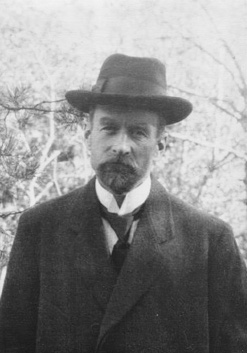
\includegraphics[width=\linewidth]{helge-von-koch.jpg}\\
      {\scriptsize\color{gray}Helge von Koch (1870--1924).
      Domaine public, Wikimedia Commons.}
    \end{column}
    \begin{column}{0.72\textwidth}
      \begin{itemize}
        \item Né à Stockholm ; élève de Gösta Mittag-Leffler, lui-même
          disciple de Weierstrass. Thèse (1892) sur les déterminants
          infinis et les équations différentielles linéaires.
        \item Succède à Mittag-Leffler à l'université de Stockholm (1911).
        \item 1901 : l'hypothèse de Riemann équivaut à une estimation
          précise de l'erreur commise en comptant les nombres premiers
          par le logarithme intégral.
        \item 1904 : « Sur une courbe continue sans tangente, obtenue par
          une construction géométrique élémentaire ».
      \end{itemize}
    \end{column}
  \end{columns}
\end{frame}

\begin{frame}{Note historique 3.1 (suite)}
  \small
  \begin{itemize}
    \item Trente ans plus tôt, Weierstrass avait exhibé une fonction
      continue dérivable nulle part (section 10) --- mais définie par
      une série trigonométrique, difficile à interpréter
      géométriquement.
    \item Von Koch voulait montrer le même phénomène par une
      construction qu'on puisse faire à la règle et au compas.
    \item Trois quarts de siècle plus tard, son flocon devient l'une des
      figures les plus connues de la géométrie fractale.
  \end{itemize}
\end{frame}
